\documentclass[main.tex]{subfiles}
\begin{document}

\section{Hardware}

With the increasing demand for highly data-parallel algorithms, and the increasing amount of data to process, hardware development started shifting towards the goal of solving that problem. Initially, that started with the increased support for vector instructions in common \acsp{CPU}, and the \acs{SIMD} model. This allowed a single instruction to operate on a set of elements at once, effectively achieving a kind of parallelism which was extremelly useful with highly data-parallel applications. Modern \intel processors, starting with the Sandy Bridge family, already support \ac{AVX} \todo{refs refs refs}, an extension to the \textit{x86} instruction set allowing \acs{SIMD} instructions capable of handling 256 bits registers. This extension also introduces three-operand \acs{SIMD} instructions that allow more general $c = a + b$ operations to be handled with a single instruction, in addition to the previous instructions which only allowed two operands ($a = a + b$).

\acs{SIMD} is also the programming model behind \acsp{GPU}, which gradually started to gain more attention for their general purpose computing capabilites. Although the hardware of a \acs{GPU} is still tightly coupled with graphics processing and rendering, there have also been several advances in their usage as \acp{GPGPU}.



\subsection{\nvidia Fermi Architecture}

The Fermi architecture was an important milestone

\begin{figure}
  \centering
  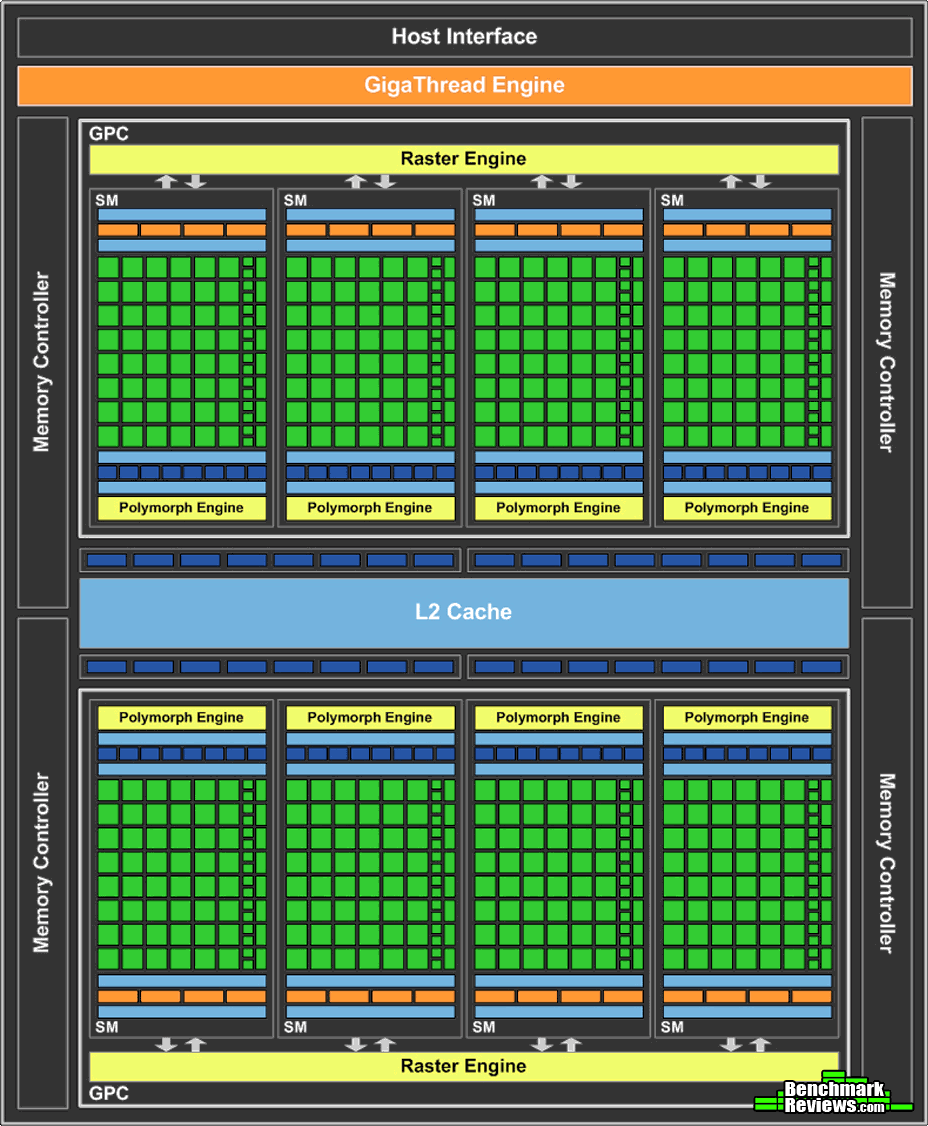
\includegraphics[width=0.6\textwidth]{arch_fermi}
  \caption{Overview of the Fermi architecture \label{fig:fermi}}
\end{figure}



\subsection{\nvidia Kepler Architecture}

\begin{figure}
  \centering
  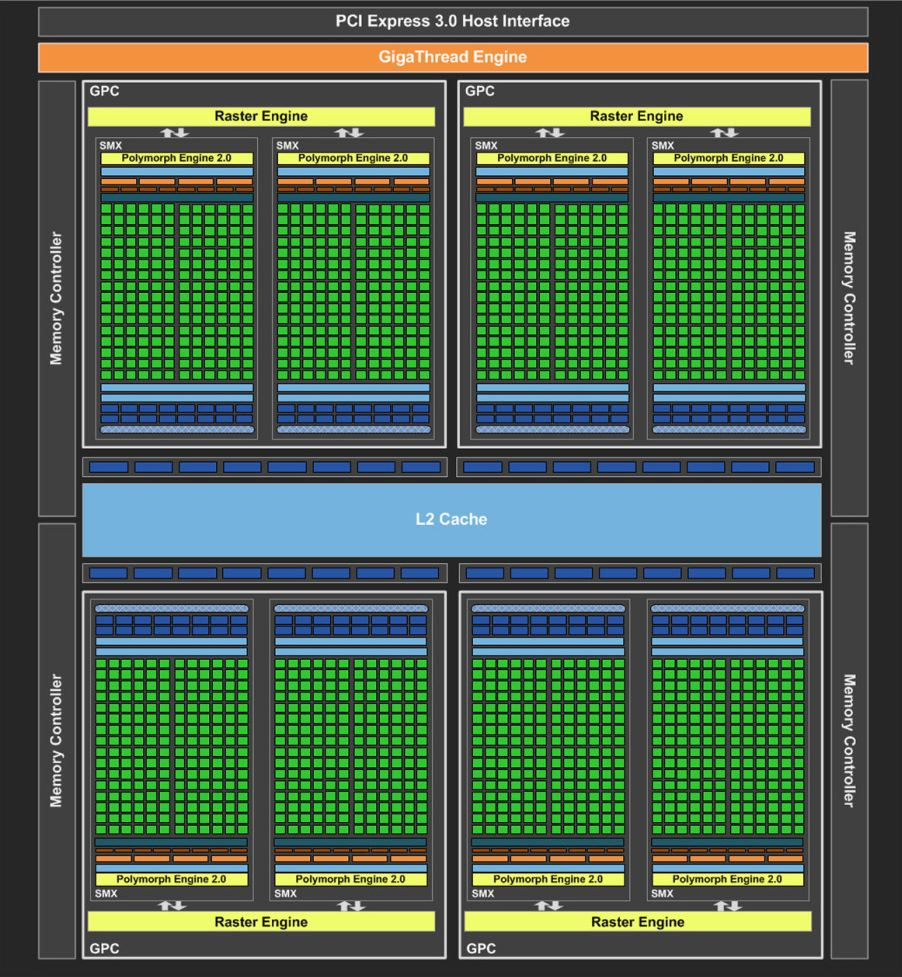
\includegraphics[width=0.6\textwidth]{arch_kepler}
  \caption{Overview of the Kepler architecture \label{fig:kepler}}
\end{figure}



\subsection{\intel Many Integrated Core}


\end{document}
